\begin{figure}[!ht]
\centering
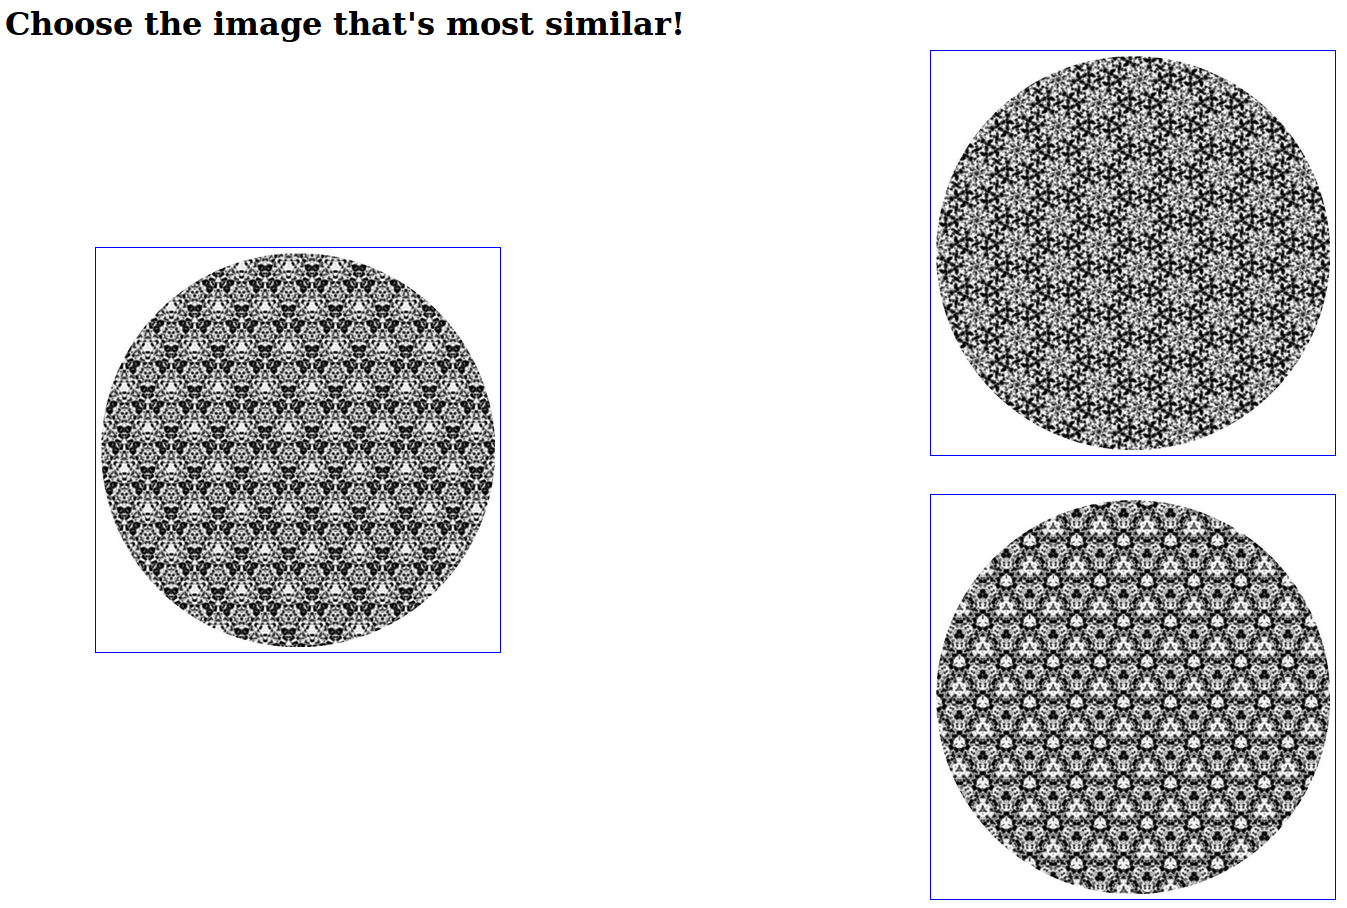
\includegraphics[width=0.9\columnwidth]{symper}
\label{screenshot}
\caption{A screenshot of the experimental task}
\end{figure}


\section{Experiments}
In order to answer these questions, we designed an experiment where people had to make a decision about which wallpaper group was which. The experiment has subjects examine three images. Two of these images have the exact same wallpaper group, and the third image is of one of the other sixteen groups. See Figure~\ref{screenshot} for a screenshot of the task given to participants. The goal of the task is to see which groups subjects can easily distinguish among and which groups are more challenging. This will allow us to examine what features of these groups cause difficulty in addition to examining whether the task itself is easy.

We recruited 106 subjects on Mechanical Turk platform to participate in the experiment for compensation. Each subject performed 272 of these types of matches. In each of these 272 tasks, there was a \textit{target} image, which is the image on the left with which they compare the other two images to. On the right, there is the \textit{goal} image, which always has the exact same group as the target image. Also, on the right is the \textit{distracter} image, which has any other wallpaper group. In the 272 tasks, each wallpaper group serves as the distracter for every other wallpaper group: thus, 272 is the simple product of 17 wallpaper groups with the 16 others.

To generate these 272 tasks, we started with five images from each wallpaper group. Then, we created every possible combination task, which is each image in each location that creates a valid task; in other words, not all three images can be of the same group. Then, each participant who accepted the HIT on Mechanical Turk was assigned a set of tasks randomly, where exactly one task had each wallpaper group as the distracter for every target image group.

We introduced a time limit of five seconds to ensure that the subjects were performing the task intuitively, rather than relying on formal knowledge. This gives participants plenty of time to click the one they feel was more similar; however, when the task was given to a few people who have education on wallpaper groups, they reported that the time limit felt too short to determine which group was which. Thus, it is fair to assume that the results we have are a result of perception rather than education.

As the task can feel long, subjects were allowed one break halfway through the experiment. Each subject was paid \$2 and a bonus for each task they successfully completed beyond chance, to encourage people to try as hard as they could on the task, instead of simply guessing. They could earn up to \$2 by answering 100\% correctly.  

Unfortunately, this incentive did not work on all participants. We excluded 10 participants from the analysis due to behavior that seemed consistent with either a lack of effort or following the directions poorly. We used three exclusion heuristics:

\begin{enumerate}
\item{A participant clicked the top or the bottom image more than 60\% of the time. If this was due to the system’s task generation, the probability of it occurring would be extremely low, about 0.001\%. However, 5/106 participants fell into this category, implying that their guessing strategy was slightly biased.}

\item{A participant had more than 20\% of their tasks time out. Over-
all, the rate of time out (exceeeding the five second time limit) was fairly low, around 4\%. Therefore, those participants with significantly higher rate of time outs either did not understand the task correctly or were not taking the task seriously. Only 4/106 participants fell into this category.}

\item{If the system registered that a participant clicked more than 125\% of the number of tasks. Each task only required a single click to complete, so the assumption is that someone who is clicking that often is not actually looking at the images before clicking. Generally, this refers to clicks on the image. While some people have a more ”excitable” clicking strategy, the average number of clicks was around 274, with the mode being 272. Those with significantly more were most likely clicking before the images loaded. Only 1/106 participants fell into this category.}
\end{enumerate}

